\chapter{Simulation Results and Discussion}
\thispagestyle{fancy}


%\section{Fractals}
%As discussed in section \ref{sec:CAandSOC}, in order to show that a dynamical system exhibits SOC, some fractal nature must be present. As done analytically for a 1-D-model in~\cite%{fractal_avalanching}, we can plot the energy of a system over time according to the definition of normalized energy
%\[
%E(t) = \int_f h(x,y,t)^2 df
%\]
%where $h$ is the height of a site at position $(x,y)$ of the field $f$ at time $t$. In MATLAB/Octave, at the end of every main loop iteration the energy is calculated:
%\begin{lstlisting}
%ee(t) = sum(sum(f.^2));
%\end{lstlisting}
%As the energy series in 1-dimensional case shows fractal properties (see~\cite{fractal_avalanching}), the question arises if this is true for a 2-dimensional case.

\section{Power-law Distributions}

In this section, investigations of the avalanche size and lifetime distributions are shown according to different boundary conditions: periodic and open.


\subsection{Periodic Boundary Conditions}

For periodic boundary conditions, no grain gets lost as long as no friction is introduced. As a consequence, the driving time and the lattice size need to be chosen carefully, in order not to run into a situation of a never-ending avalanche. Also, to analyze the distribution, good statistics must be present - a reasonably large lattice is needed. Although, theoretically, the lattice is of infinite size (due to its periodic nature), which implies that the size should not matter.

Here, a $100\times 100$ lattice is studied with a driving time $T=5000$. The results are presented in the figures~\ref{sp}. The power-law behaviour is easily recognizable for the avalanche size and for the avalanche lifetime, although the latter fit is of poorer quality.

The first point of both plots correspond to the case where no avalanches occur. It is included to show that the system stays subcritical most of the time, and only sometimes becomes overcritical. 


\begin{figure} 
\begin{center}
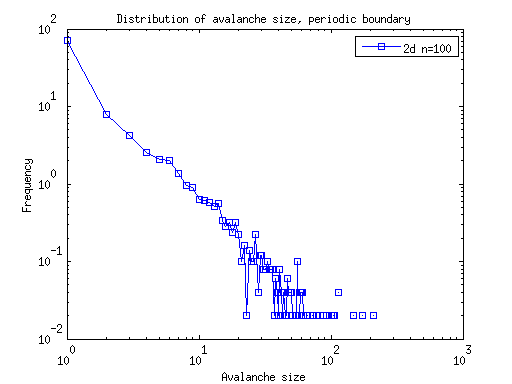
\includegraphics[width=0.75\textwidth]{results/sp.png} \\
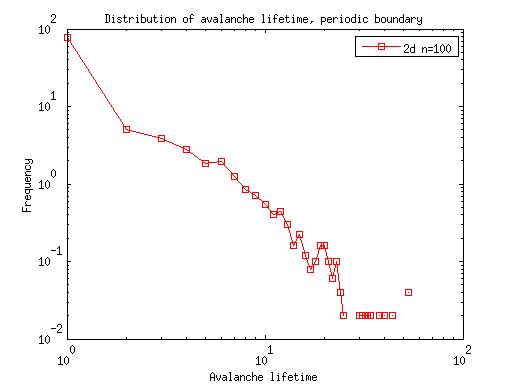
\includegraphics[width=0.75\textwidth]{results/tp.png} 
\caption{Avalanche size and lifetime distribution for a $100\times100$ lattice, with periodic boundary conditions. 
The driving time is $T=5000$.  }
\label{sp}
\end{center}
\end{figure} 

Higher dimensions are not treated here, due to high memory and simulation runtime requirements. As real systems are finite and dissipative, the periodic boundary case without grain loss is not of much interest, i.e. it is not considered a SOC phenomenon. Instead, a friction parameter is introduced and discrete grain addition is replaced by a continuous one, thus replacing the integer field by a \emph{real} field and presenting a more realistic model.

The periodic boundary in principle implies lattice size independence, which will represent a computational advantage, as a small lattice can be chosen.

Results of this situation for $d=2$, with $n=10$, $n=50$ and $n=100$ are shown in figures~\ref{spf1} and~\ref{spf2}. A clear cut-off for large avalanche number due to friction is seen, but with a nice power-law distribution for small avalanches. The lifetime is not shown as it does not differ much from the case in figure~\ref{sp}. For the case of $n=100$, the simulation is run ten times longer than for the other cases, resulting in a distribution different from small or medium-size ones for large avalanches.


\begin{figure} 
\begin{center}
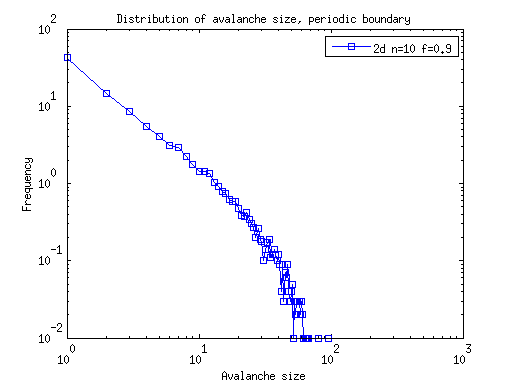
\includegraphics[width=0.75\textwidth]{results/spf.png}
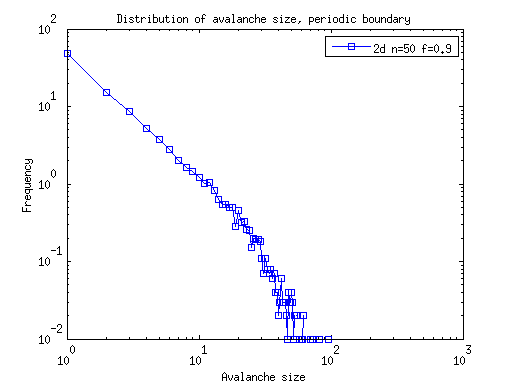
\includegraphics[width=0.75\textwidth]{results/spf50.png} \\
\caption{Avalanche size distribution for a $2d$ lattice with friction and periodic boundary conditions. The driving time is $T=10\,000$ and the lattice size is $n=10$ and $n=50$, respectively. }
\label{spf1}
\end{center}
\end{figure}


\begin{figure} 
\begin{center}
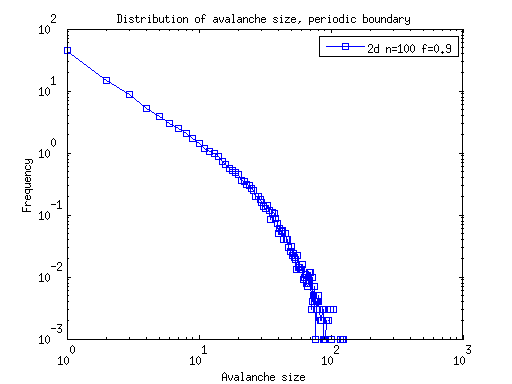
\includegraphics[width=0.75\textwidth]{results/spf100a.png}
\caption{Avalanche size distribution for a $2d$ lattice with friction and periodic boundary conditions. The driving time is $T=100\,000$. }
\label{spf2}
\end{center}
\end{figure} 

The importance of the dissipation becomes clear as the critical exponent changes for different values of friction.

From figures~\ref{spf1} and~\ref{spf2} we can conclude that small lattices can also be used with a small driving time, saving computational capacity. Therefore, this case will be used to explore higher dimensional lattices, that are computationally more costly. Figures~\ref{dspf3} and~\ref{dspf4} show the results of the $3d$ and the $4d$ case respectively. The cut-off effect due to friction is much less than for the $2d$ lattice. The effect of an increase in the friction value is shown in figure~\ref{3spf}. From this analysis, clearly, the dissipation plays an important role. Nevertheless, \emph{on average}, the total energy of lattice is kept constant when the system evolves (see figure~\ref{ep}). Furthermore, for $d=1$, no power-law behaviour is seen, in agreement with the prediction of theory presented in~\cite{soc} (the situation for open boundary has also been checked to be the same). Refer to figure~\ref{1p} for the results.


\begin{figure}
\begin{center}
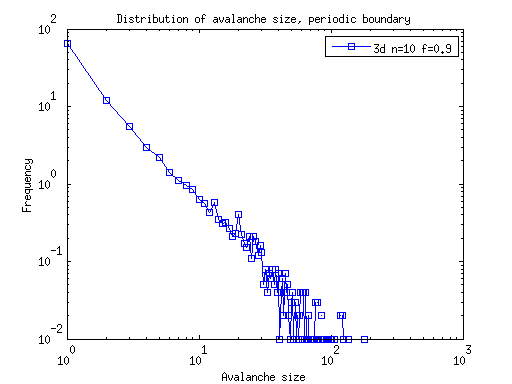
\includegraphics[width=0.75\textwidth]{results/3spf.png} \\
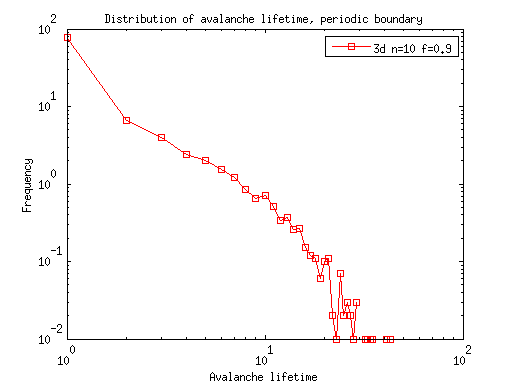
\includegraphics[width=0.75\textwidth]{results/3tpf.png} \\
\caption{Avalanche size and lifetime distribution for a $3d$ lattice with friction and periodic boundary conditions. }
\label{dspf3}
\end{center}
\end{figure}

\begin{figure}
\begin{center}
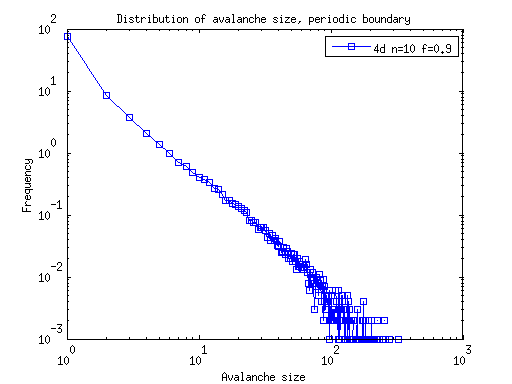
\includegraphics[width=0.75\textwidth]{results/4spf.png} \\
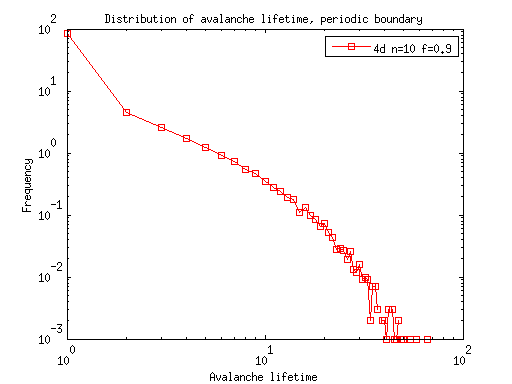
\includegraphics[width=0.75\textwidth]{results/4tpf.png} \\
\caption{Avalanche size and lifetime distribution for a $4d$ lattice with friction and periodic boundary conditions. }
\label{dspf4}
\end{center}
\end{figure}


\begin{figure}
\begin{center}
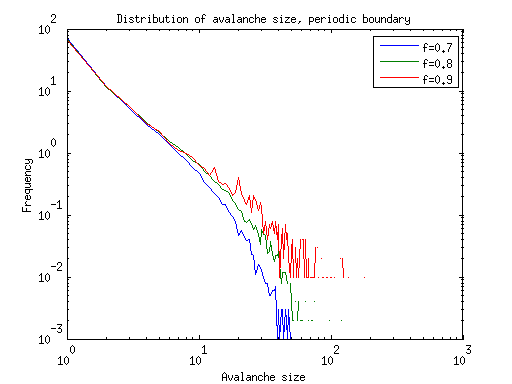
\includegraphics[width=0.75\textwidth]{results/3spfmulti.png}
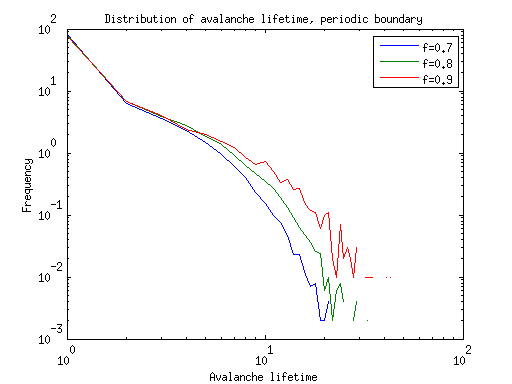
\includegraphics[width=0.75\textwidth]{results/3tpfmulti.png}
\caption{Avalanche size and lifetime distribution for a $3d$ lattice with different friction parameters using periodic boundary conditions. The smaller the friction parameter, the larger the dissipation. The first point in the lifetime distribution corresponds to ``zero avalanches'' during the lifetime. }
\label{3spf}
\end{center}
\end{figure}


\begin{figure}
\begin{center}
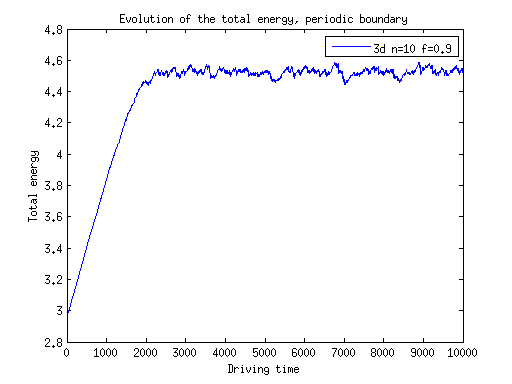
\includegraphics[width=0.75\textwidth]{results/3ep.png}
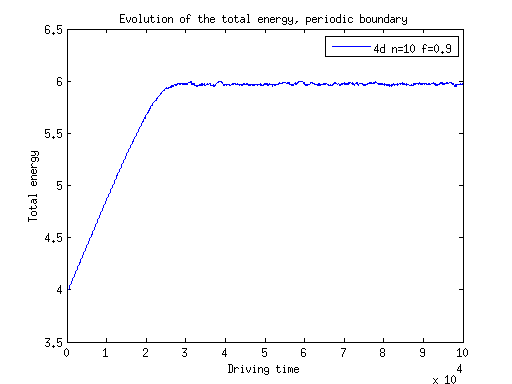
\includegraphics[width=0.75\textwidth]{results/4ep.png}
\caption{Normalized total energy evolution for $3d$ and $4d$ lattices with friction and periodic boundary conditions. }
\label{ep}
\end{center}
\end{figure}


\begin{figure}
\begin{center}
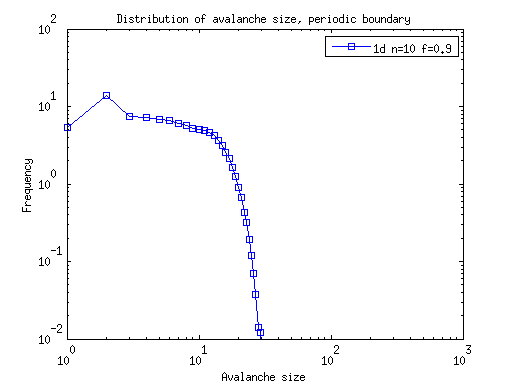
\includegraphics[width=0.75\textwidth]{results/1sp.png}
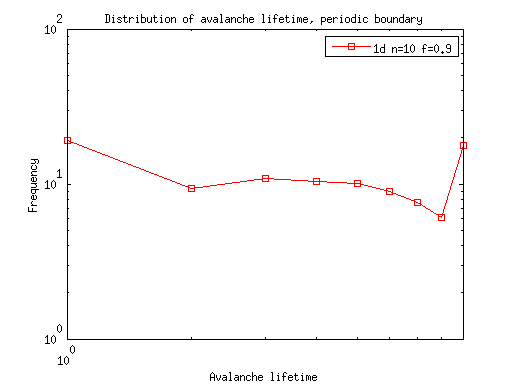
\includegraphics[width=0.75\textwidth]{results/1tp.png}
\caption{Avalanche size and lifetime distribution for $1d$ lattices with friction, periodic boundary conditions and $T=100\,000$. There is no criticality for this case. }
\label{1p}
\end{center}
\end{figure} 










\subsection{Finite boundary conditions}

A perturbation in the boundary might cause a different avalanche distribution than a perturbation placed in the bulk. One might expect a bulk perturbation to produce bigger avalanches, as the grain has to be transported further in order to be lost at the boundaries.

Here, this effect is studied for 2-dimensional case and remarkably, different avalanche size distributions can be seen (figure~\ref{sv}). Furthermore, the high dispersion in large avalanche sizes for the bulk case causes a worse power-law fit compared to the boundary perturbation case.

\begin{figure} 
\begin{center}
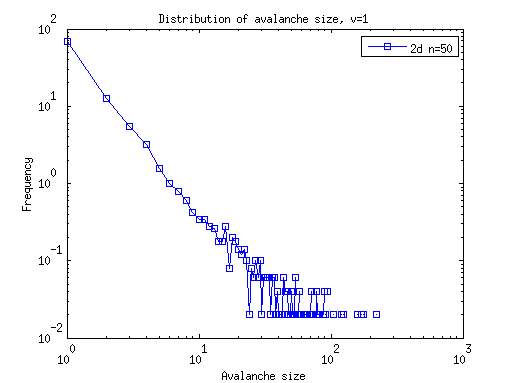
\includegraphics[width=0.75\textwidth]{results/sv1.png}
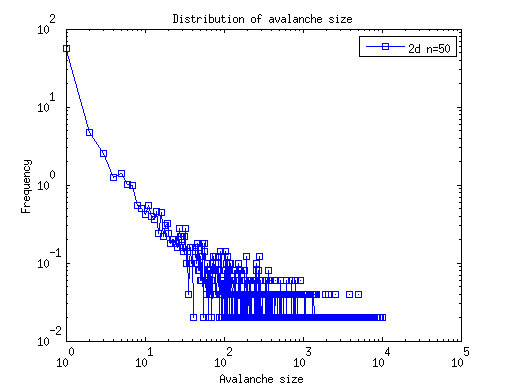
\includegraphics[width=0.75\textwidth]{results/sbulk.png} 
\caption{Avalanche size distribution for a $50\times50$ lattice for different perturbation sites (first plot: site $(1,1)$, upper left the corner; second plot: bulk site, $(25,25)$). The driving time is $T=5000$.}
\label{sv}
\end{center}
\end{figure} 

For random perturbation sites, the result is closer to the bulk one than to the boundary one.


The relation of the number of sites in the volume to the number of sites at boundary should be proportional to the lattice size $n$, as it is basically the ratio of volume and area. This implies that on a large lattice one encounters more large avalanches than on a smaller lattice. See figure~\ref{sn}.

\begin{figure}
\begin{center}
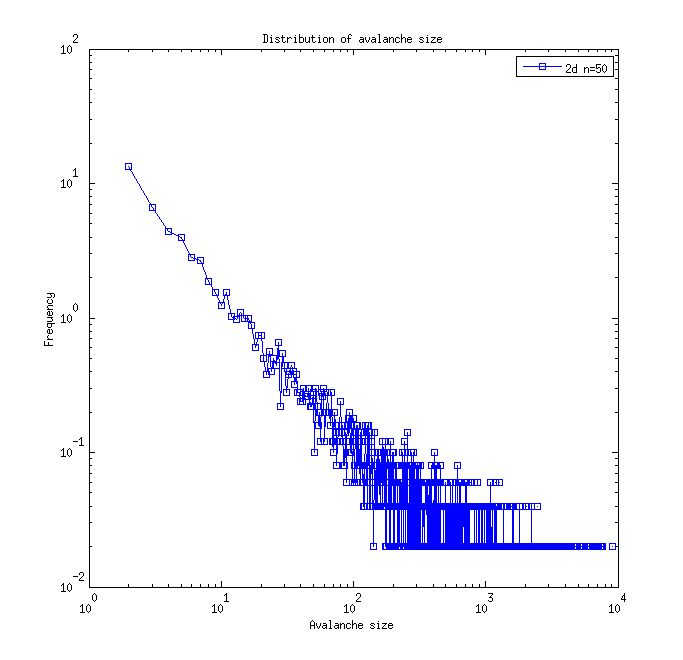
\includegraphics[width=0.75\textwidth]{results/2sn50.png}
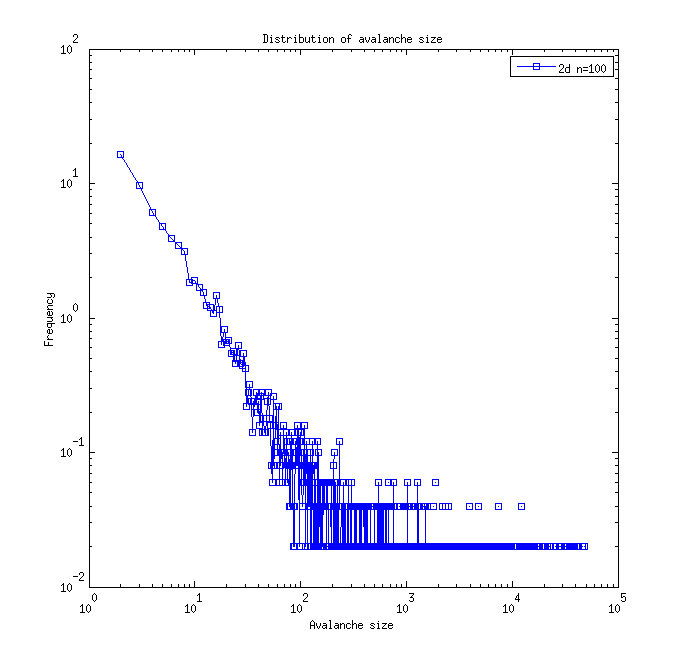
\includegraphics[width=0.75\textwidth]{results/2sn100.png}
\caption{Avalanche size distribution for $2d$ lattices with different sizes and open boundary conditions.}
\label{sn}
\end{center}
\end{figure} 

Adding friction (and thus going to a more realistic case), the number of large avalanches reduces as seen in figure~\ref{so}. Again, friction is crucial for generating a power-law like distribution and for the cut-off effect discussed before.

\begin{figure}
\begin{center}
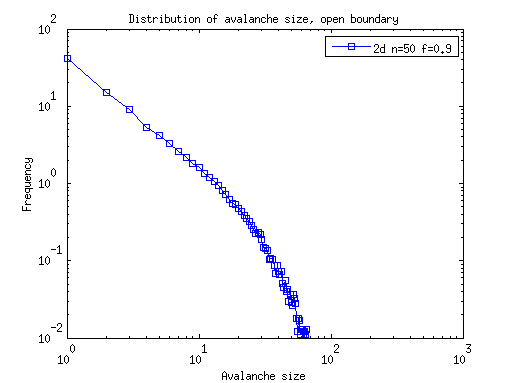
\includegraphics[width=0.75\textwidth]{results/2sof.png}
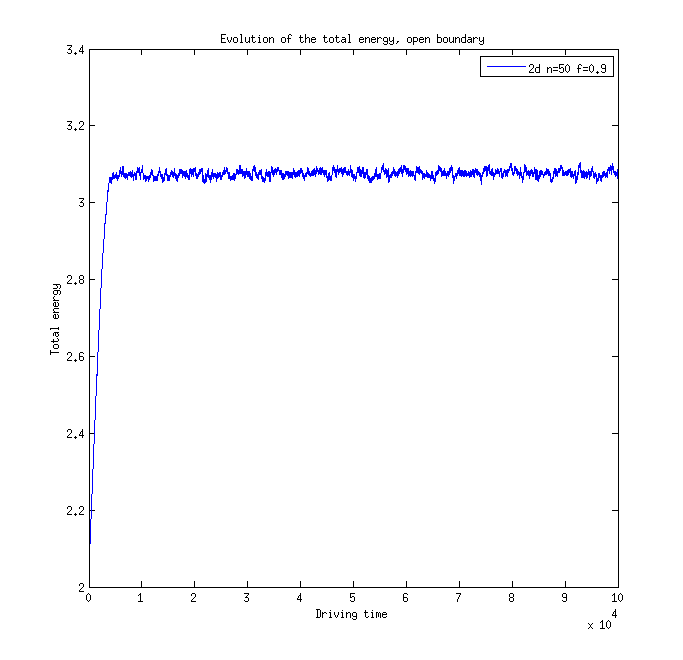
\includegraphics[width=1\textwidth]{results/2eof.png}
\caption{Avalanche size distribution and energy evolution for a $2d$ lattice with friction and open boundary conditions.}
\label{so}
\end{center}
\end{figure} 


During the driving time, the energy of the system, namely the sum of the values of the field of all sites,
tends to oscillate around a constant value, as the additional grain in each driving time is compensated with the dissipation during avalanche,
see figures~\ref{so} and \ref{ep}.





\subsection{Distribution for small lattices}


The total number of possible configuration states containing only one ovecritical site is equal to
\[
N_c=n^d\times (2d)^{n^d-1}
\]
A chain of size $n^d$ linearizes the lattice. One site is fixed equal to the critical value, i.e. the minimal value that the site will topple, set as $E_c=2d$ for convenience. The rest of the ($n^d-1$) sites can have any value from $\{0,1, \ldots, 2d-1\}$, so $2d$ values.

However, not all of these configurations will appear during the driving time. As only one energy grain is randomly added to the system for each driving time,
and as the system can dissipate grains, this will soon lead to a characteristic average energy value per site, as discussed before. For example, configurations such that all sites are zero except the overcritical one will never occur, unless it is started with. Thus, only a finite subset of the possible set $A$ will occur during one simulation (subset of $A$).
The avalanche phenomenon, a set of configurations with one or more overcritical site(s), indeed creates a relation of the subset of $A$ with a subset of subcritical configurations $B$. In contrast, the driving time (the grain adding) makes the system critical, therefore creating the relation $B \to A$.

Because of the discrete nature of the lattice, all these relations between the discussed two sets $A$ and $B$ exist independently if the system is run or not.
Although running the system restricts the results to only a certain part of the full distribution.

The avalanches can be characterized by their size (the total number of sites that became overcritical)
or by their lifetime (the number of different configurations with some sites overcritical). By definition,
the values that the size can have are bigger than the values of the lifetime (as the former refers to the number of \emph{sites}, and the latter, to the intermediate \emph{configurations}).

For clarification, the avalanche size and lifetime distribution of a simple case of a small lattice with finite boundary is shown in figure~\ref{multi}.
The initial configuration is \textbf{minimally stable}, i.e. all sites have a value $E_c-1$, meaning that one grain addition in any of the site will lead to a \emph{catastrophic} avalanche that will affect the whole system.
We might consider these distributions as \emph{exact} (the subset of 1 state overcritical configurations is almost the whole set, as the system is small enough),
as they do not change after running the simulation for even longer time.
These distributions are more exponetial-like ($y=c^{-x}$) than power-law-like.

\begin{figure}
\begin{center}
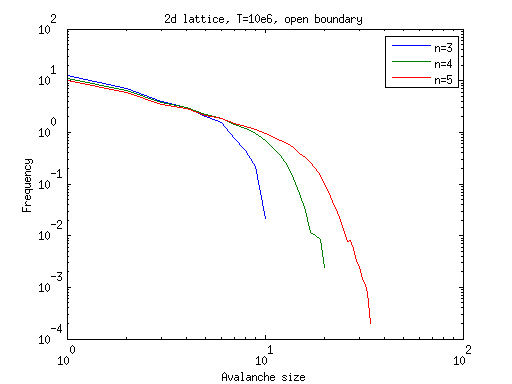
\includegraphics[width=0.75\textwidth]{results/smulti.png}
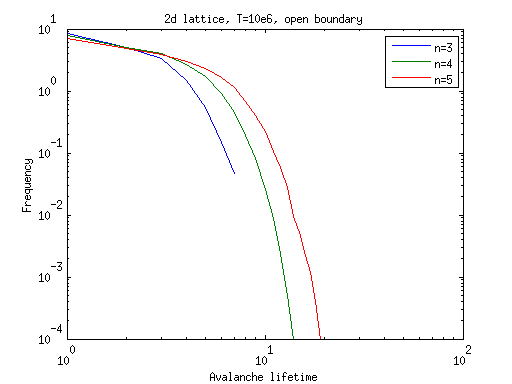
\includegraphics[width=0.75\textwidth]{results/tmulti.png}
\caption{Avalanche size and lifetime distribution for small $2d$ lattices,
which started with all the sites critical.
These distributions are checked to fit quite well with exponential decaying distributions. The fitting parameters are not shown, as their values are not meaningful for the discussion.}
\label{multi}
\end{center}
\end{figure}

What happens for larger lattices is that the size of the avalanche is restricted to the small and middle ones, so in some sense the power-law distribution is an approximation for this regime. Catastrophic avalanches that affect to the whole system never happen, except one is imposed as an initial configuration.
A zero configuration will neither evolve to the minimally stable state (that leads to catastrophic events).

To check this idea, a bigger lattice of $50\times 50$ is run in 2 dimensions with a total driving time of $T=1\,000\,000$.
The result of avalanche size distribution is shown in figure~\ref{sfit}, with a respectable power-law fitting over two decades.

\begin{figure}
\begin{center}
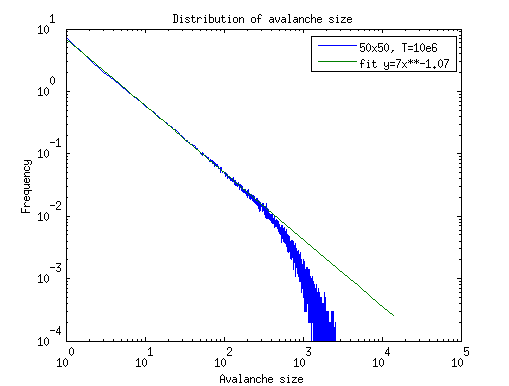
\includegraphics[width=0.75\textwidth]{results/2dsfit.png}
\caption{Avalanche size distribution for a $2d$ lattice. }
\label{sfit}
\end{center}
\end{figure}

The catastrophic avalanches would have a size of order $10^4$, occurring for minimally stable states, which will have an average energy per site of
\[
<E>=(n^d(E_c-1)+1)/n^d=E_c-1+1/n^d
\]
For a large lattice, it is $<E>\sim E_c-1$, so $3$ for this case. The system evolves to an average energy per site around $2$ (see figure~\ref{2e}, which starts with a random initial configuration. Starting with a minimally stable state would converge to the same value).
Therefore, many theoretically possible states must be strongly suppressed.
A small remnant which is not power-law-like stays. One might first consider it as a finite size effect,
but it is indeed a discrete effect, as it will remain for any lattice size if the simulation is run long enough.
This is due to the fact that the system is intrinsically discrete.

\begin{figure}
\begin{center}
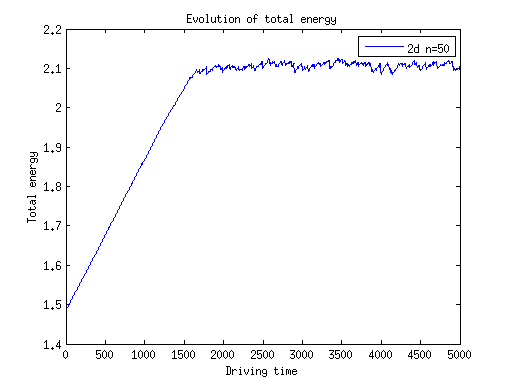
\includegraphics[width=0.7\textwidth]{results/2e.png}
\caption{The evolution of the total energy per site for $2d$ lattice, starting with a random configuration. }
\label{2e}
\end{center}
\end{figure}

Nevertheless, if the system is continuous, which cannot exactly be reproduced with a computer simulation,
then an infinite number of possible configurations would occur while running the simulation for an infinitely large time and the result should give a power-law distribution.
Of course, this is a hypothesis and should be proven mathematically, which is not part of this project.
Our discussion is at the qualitative level, aiming to help understanding why sandpile models generate power-law-like distributions.

Previous plots showed an accumulated large amount of large events, but also with a lot of dispersion which is mainly statistical fluctuations. Running for long enough time, this effect should disappear and a distribution like the one in figure~\ref{sfit} should come out, comparing with the plots in figure~\ref{sn}, where $T$ s much smaller.

\vspace{1em}

As seen in all the different cases studies here, the lifetime distribution always keeps the same shape.
The catastrophic avalanches do not have the largest lifetime and normally, the largest lifetime value is much less than the total number of sites. The avalanche size can in contrast outnumber it.
Table~\ref{tabn2} shows catastrophic avalanches in a 2-dimensional lattice. The maximum avalanche size is of the order $n^d$, where the lifetime is of the order $n\cdot d$.
Therefore, lifetime should converge faster than size.

\begin{table}
\begin{tabular}{|c|c|c|c|}
 \hline
 n & site & av. size & av. lifetime\\ \hline
 3 & (1,1) & 9 & 5 \\ 
                    & (1,2) & 9 & 4 \\ 
                    & (2,2) & 10 & 3 \\ \hline
 4 & (1,1) & 16 & 7 \\ 
                    & (1,2) & 16 & 6 \\ 
                    & (2,2) & 21 & 5 \\ \hline
 5 & (1,1) & 25 & 9 \\ 
                    & (1,2) & 25 & 8 \\ 
                    & (1,3) & 25 & 7 \\ 
                    & (2,2) & 34 & 7 \\ 
                    & (2,3) & 34 & 6 \\ 
                    & (3,3) & 35 & 5 \\ \hline
\end{tabular}
\caption{Table with catastrophic avalanches, where the \emph{site} refers to the critical site, while other sites are minimally stable (with value $E_c-1$).}
\label{tabn2}
\end{table} 

\vspace{1em}

If one grain is always placed onto the same site at each driving time, this will lead to a \emph{limit cycle}, where a finite set of configurations will keep repeating themselves. These states are called \emph{recurrent states}.



The existence of limit cycles is proven analytically using the abelian property in \cite{deepak}, and is also checked it for small lattices, for example
\[ \left[ \begin{array}{ccc}
3 & 2 & 2 \\
3 & 4 & 3 \\
0 & 1 & 3 \end{array} \right] .
\]
Adding a grain to the center constantly leads to a repeating but finite number of configurations, which can be checked by hand or using the the \mcode{abelian_sandpile.m} program. In fact, this happens to any initial configuration attracted by the corresponding limit cycle (many different limit cycles exist depending on where the grain is placed).
Furthermore, for the periodic boundary condition, with only one grain the system will go into an infinite loop between these configurations. Using randomized grain adding avoids such situations.











